\section{Test proposal at FZK}
Proposal for InfiniBand testing in FZK

\subsection{Future DAQ for FAIR}
The experiments planned for the upcoming new facility FAIR at GSI require a new generation
of data acquisition systems. As an example we consider the Compressed Baryon Matter experiment CBM.
The data acquisition for this experiment requires fast building network technologies,
capable to transport and switch enormous amount of data in real time. The main task of the event building
network (BNet in fig. \ref{fig:test-daq-all} is to combine data of one (or several) events in one computer node,
where special filtering algorithms can be performed to accept or reject the event for further physical analysis.
These algorithms require almost all data of an event. Therefore a triggerless DAQ is envisioned.
All data items are time stamped. The time stamps are then used to define the events and determine the data of an event.
Experimental data flow from the many detector subsystems continuously in parallel into the event building net. They should be
resorted according their time stamps or event tags. Actually, we need a logically network with many ($\sim$1000) nodes, where each
node should be able to exchange data with any other. Beside the main data traffic one expects to have meta
data, which should be transported over the same network: flow control and transfer scheduling data.
SystemC simulation was done to investigate different possibilities for traffic patterns.
\begin{figure}[htb]
\centering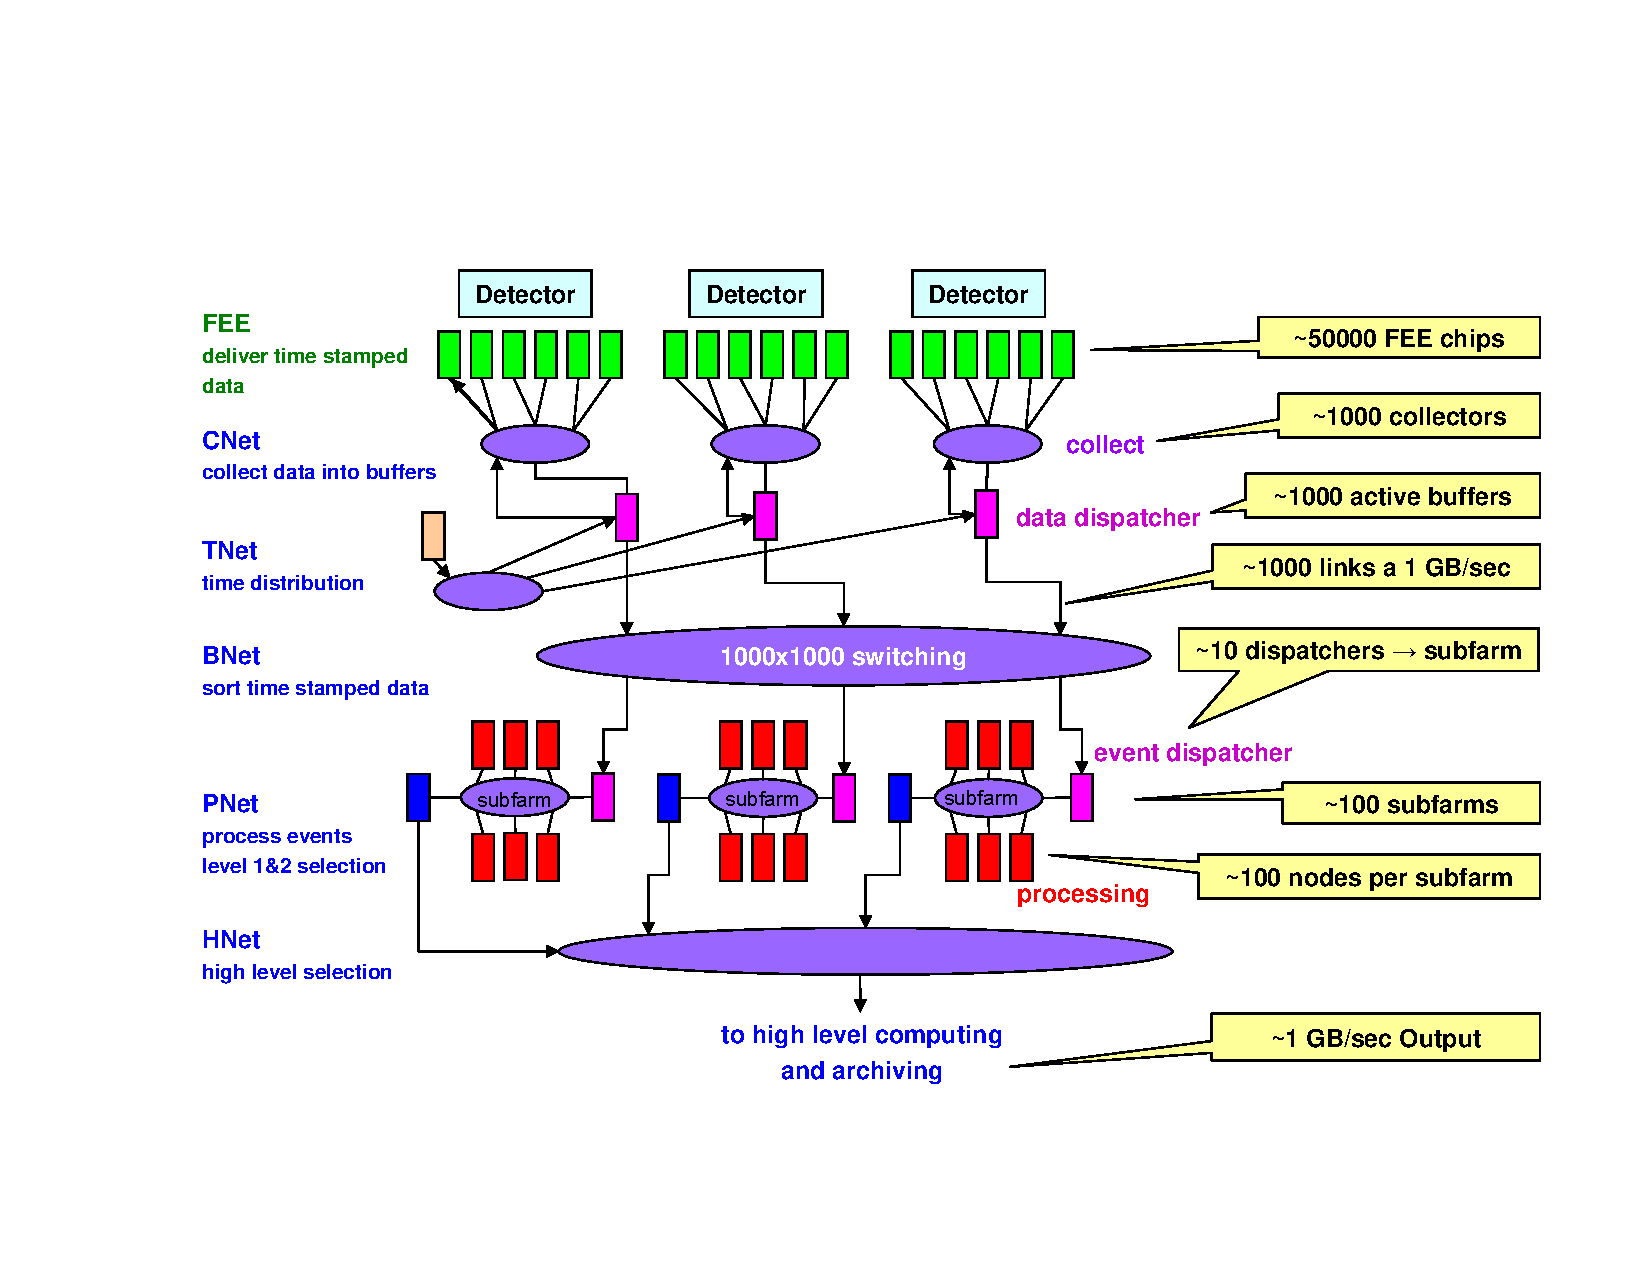
\includegraphics[width=.8\textwidth]
{dabcf-daq-all}
\caption{CBM overall data processing architecture}
\label{fig:test-daq-all}
\end{figure}


\subsection{Infiniband cluster in GSI}
At the preliminary phase we consider InfiniBand as possible candidate for such a building network.
For investigation of InfiniBand and communication protocols a 4-nodes cluster was established
at GSI since November 2005. Each node consists of a Double Opteron machine, equipped with Mellanox
MHES18-XT (PCIe) host adapters. For connectivity a Mellanox MTS2400 switch was used.

\subsection{IBGold and uDAPL tests}
At the beginning we have installed and use Mellanox IBGold 1.8.0 package.
uDAPL was taken as main data transport protocol.
The main features of uDAPL are: point-to-point communications, zero-copy data transfer and remote DMA.
A C++ library was implemented to wrap the main functionality of uDAPL in more convenient form for usage in test programs.

A mechanism to synchronize the clocks of the nodes was implemented.
It uses small round-trip packets between master and all slave nodes.
Each round-trip packet takes about 12 $\mu$s. The master calculates the clock difference
and submits correction coefficients (time shift and scale) to all nodes at the end.
One achieves a clock synchronization between nodes with a precision of a few $\mu$s
per 100 seconds. For long-time tests the time synchronization routine must be repeated regularly.

A scheduled data transfer mechanism was implemented. Scheduled transfer means that each
nodes gets a predefined traffic pattern, where transfer buffer size, target node and
exact sending time are specified. In the test applications always full connectivity is
established, therefore arbitrary traffic patterns can be tested. Several patterns
were investigated: one-to-all, all-to-one, all-to-all (several variations).
For us all-to-all performance is of main interest while it corresponds to the
expected traffic pattern of the CBM event building net.

We also have investigated non scheduled data transfers.
In this case the data transfer is not synchronized between nodes.
Each node just sends packets in each direction until the
sending queue will be filled completely. The result of both tests are represented in the table \ref{test-xmit-table}.
More detailed results can be found in the following sections.

\begin{table}[h]
\begin{tabular}{|p{3.0cm}|p{1.0cm}|p{1.0cm}|p{1.0cm}|p{1.0cm}|p{1.0cm}|p{1.0cm}|p{1.0cm}|p{1.0cm}|p{1.0cm}|}      \hline
Buffer & 1K & 2K & 4K & 8K & 16K & 32K & 64K & 128K & 256K \\ \hline
Scheduled & 247 & 437 & 705 & 877 & 910 & 936 & 948 & 953 & 954 \\ \hline
Chaotic & 273 & 524 & 776 & 889 & 923 & 937 & 947 & 953 & 954 \\ \hline
\end{tabular}
\caption{Receive data rates (in bytes/$\mu$s) in IBGold uDAPL all-to-all tests}
\label{test-xmit-table}
\end{table}
One can see that above 16K buffers the transfer rate exceeds 900 bytes/$\mu$s.
One should also take into account, that the total throughput over each InfiniBand
host adapter is two times bigger because each node receives and sends data simultaneously.
We also observe that the resulting data rate depends from the size of sending and receiving queues (not shown here).

One can see that chaotic transfer (no schedule) is faster for small packets sizes.
Actually, with older firmware, we observed a much bigger difference.
The advantage of chaotic traffic is that it does not require additional
time synchronization between send operations. But it is still not clear if such
approach will work on bigger system with many nodes.

\subsection{OFED and verbs tests}
In November 2006 we start investigation of new OFED 1.1 package, provided by OpenFabrics Alliance (openfabrics.org). As Mellanox IBGold package, it includes all required drivers and protocols for
working with InfiniBand clsuters. Actually, this package becames an official development line for Mellanox
and will replace IBGold in the future.

First we have tested uDAPL from OFED package. Results shown in table \ref{test-ofeddapl-table}.

\begin{table}[h]
\begin{tabular}{|p{3.0cm}|p{1.0cm}|p{1.0cm}|p{1.0cm}|p{1.0cm}|p{1.0cm}|p{1.0cm}|p{1.0cm}|p{1.0cm}|p{1.0cm}|}      \hline
Buffer & 1K & 2K & 4K & 8K & 16K & 32K & 64K & 128K & 256K \\ \hline
Scheduled & 264 & 490 & 700 & 788 & 835 & 866 & 875 & 879 & 880 \\ \hline
Chaotic & 309 & 536 & 688 & 788 & 838 & 868 & 878 & 881 & 882 \\ \hline
\end{tabular}
\caption{Receive data rates (in bytes/$\mu$s) in OFED uDAPL all-to-all tests}
\label{test-ofeddapl-table}
\end{table}

Results looks similar to IBGold, but there is other upper limit of achievable
bandwidth 880 bytes/$\mu$s instead of 954. This limitation appears only for
all-to-all communication and must be investigated separately. For all-to-one
and one-to-all with OFED we achieved data rates up to 985 bytes/$\mu$s, which
is better than 972 bytes/$\mu$s with IBGold.

With OFED we also have tried another library - libibverbs. This protocol
allows programs to use InifiniBand "verbs" for direct access to IB hardware
from userspace. Main advantage of verbs compared to uDAPL is the support of multicast
data transfer, missing in uDAPL API. While uDAPL interface is very similar to verbs,
we design common light-weight C++ interface for both uDAPL and libibverbs.
This allows us to run same performance tests with "verbs" too.
Actually, results of "all-to-all" tests were not much different from uDAPL ones.
Only for small packets we achieve better performance - 365 bytes/$\mu$s for 1K buffers.

We also extend functionality of our C++ interface to be able work with multi-cast data transfer.
Achieved performance of multi-cast transfer was 625 bytes/$\mu$s for 2K buffer size.
A drawback of multi-cast is the unreliable protocol behind; therefore packet lost should be taken into account.
On our cluster we observe maximum 0.002\% portion of lost packets for multi-cast-only transfers.

With the multi-cast we were able to test traffic patterns, similar to that was simulated with SystemC.
Such pattern mixes normal all-to-all data transfer (~90\%) with additional flow control traffic (~10\%).
Controlling traffic includes point-to-point slave-controller communications and multi-cast traffic
from controller to all slaves.
For 8K buffers we achieve 750 bytes/$\mu$s of main data traffic and 23 bytes/$\mu$s of multi-cast traffic.
And we see no multi-cast packets lost.


\subsection{Planned test in FZK}
\subsubsection{One switch}
First, we would like to repeat the same communication tests on a bigger cluster
in scope of single InfiniBand switch (switch module). We would like to test,
how network performance (data throughput over each connection) depends from
the number of active nodes. And also it is interesting to see if chaotic transfer
still as efficient as scheduled traffic. 12-24 nodes should be enough for such kinds of test.
\subsubsection{Switch fabric}
Second, we would like to test all-to-all communication on a switch fabric,
where more than one switch (switch module) is involved. In that case it is interesting
if correct traffic scheduling gives an advantage or if one can keep a simple round-robin
scheme or even non-scheduled transfer at all.
\subsubsection{Big cluster}
Third, our special traffic pattern with small portion of multi-cast traffic
would be interesting to test on a relatively big system. Do we get same
performance as for small system, how much multi-cast packets will be lost,
can we implement simple retry algorithm for them?


\subsection{System requirements}

For usage of uDAPL (in IBGold or OFED) following components are required:
\begin{compactitem}[$\bullet$]
\item uDAPL library - libdat.so
\item uDAPL includes - "dat/udat.h"
\item configured IPoIB - required by uDAPL to establish connections
\item user account and ssh (or rsh) to run application
\end{compactitem}

For usage of libibverbs and multi-cast in OFED:
\begin{compactitem}[$\bullet$]
\item verbs library - libibverbs.so
\item verbs includes - "infiniband/verbs.h"
\item Open Subnet Manager (OpenSM) libraries - libopensm.so libosmcomp.so losmvendor.so
\item opensm includes - "vendor/osm\_vendor\_api.h" "vendor/osm\_vendor\_sa\_api.h"
\item user account and ssh (or rsh) to run application
\end{compactitem}
